% ==============================================================================
%
%                             Mission
%
% ==============================================================================
\chapter{Mission} \label{chapt:mission}
The following sections will first cover the starting point based on appendix \ref{app:aufgabenstellung} and the available resources (appendix \ref{app:technicial_requirements}). Different possible solutions will be covered in \ref{chapt:solutions} before presenting the concept in \ref{chapt:mission:concept}. \\

In a world of self driving cars and virtual reality, having a digital copy of
the real world yields several benefits. Cars can be trained in a virtual city
to increase the performance of their algorithms and video games could get more
realistic if the player could walk through the streets of a major city. Gathering this data is one problem and processing the images is another. Pictures have to be converted, analyzed and processed. This requires a great deal of computational power for a task that is repeated several times.

% ==============================================================================
%
%                             Starting Point
%
% ==============================================================================
\section{Starting Point}
To accelerate intense image processing a dedicated hardware approach is investigated. To do so, a basic image processing algorithm such as the Wallis filter is implemented in an FPGA that communicates over a network with a host computer. The image processing task should later be distributed onto multiple FPGAs to accelerate the processing even more \cite{nomokoReqs}. Before listing possible solutions the available resources need to be dissected.

\subsection{FPGA Board} \label{chapt:mission:fpgaboard}
\begin{figure}[tb!]
    \centering
    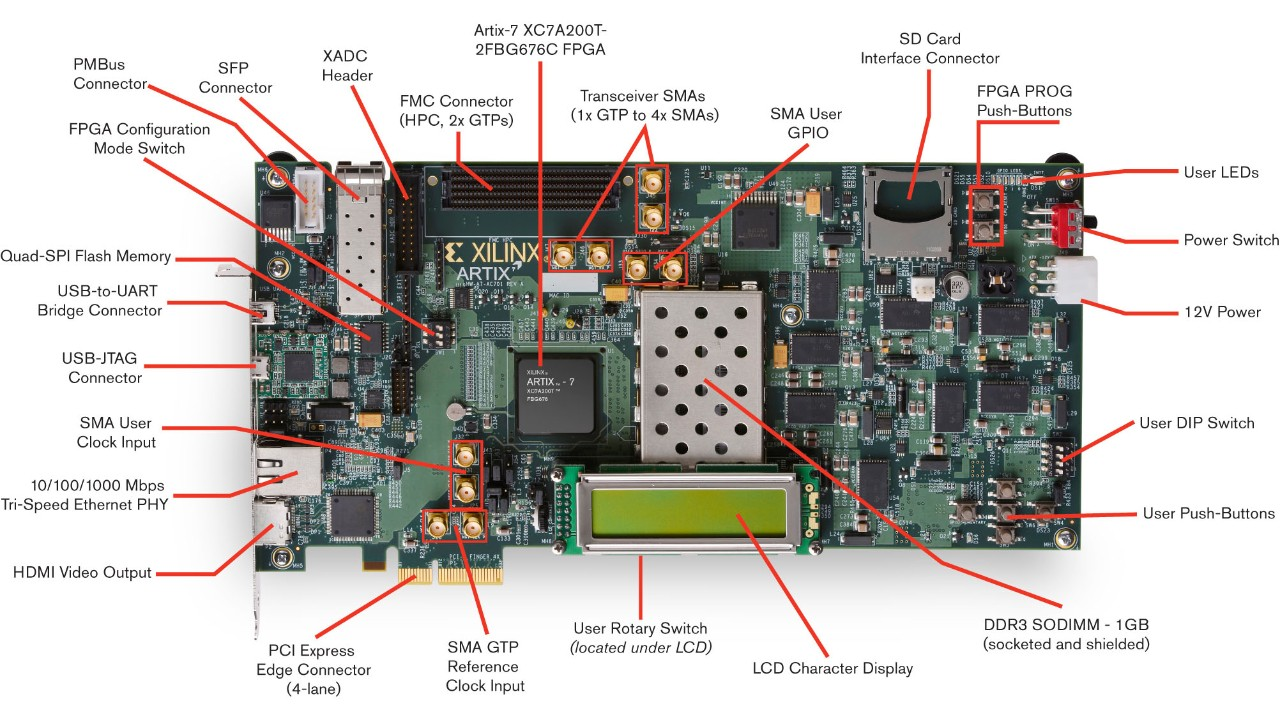
\includegraphics[width=\textwidth]{images/mission/ac701.png}
    \caption{Xilinx AC701 Evaluation Kit \cite{image_ac701}}
    \label{fig:ac701}
\end{figure}

The Xilinx AC701 Evaluation Kit is used as development platform. It features an
Artix-7 FPGA and several useful on-board peripherals. The JTAG interface is used
for configuration and debugging of the FPGA. To connect the platform to the
network, a Gigabit Ethernet PHY handles the first layer of the OSI model in
hardware (see chapter \ref{chapt:theory:physical}). Storing data is possible in the DDR3 memory
module. Table \ref{tab:ac701} shows a summary of the important peripherals on
the AC701 board.
\\
\begin{table}[b!]
    \centering
    \begin{tabular}{l l}
        \toprule
        Part & Description \\
        \midrule
        FPGA & XC7A200T-2FBG676C \\
        JTAG & Onboard JTAG configuration circuitry to enable configuration over USB \\
        Memory & DDR3 SODIMM 1GB up to 533MHz / 1066Mbps \\
        Ethernet & 10/100/1000 Mbps Ethernet (RGMII) \\
        \bottomrule
    \end{tabular}
    \caption{Xilinx AC701 key board features \cite{xilinx_ac701}}
    \label{tab:ac701}
\end{table}

The XC7A200T FPGA is part of the Artix-7 family. It is optimized for high logic
throughput at low costs. Important for this project is the number of logic cells
and the amount of on-chip memory. With more logic cells available, data can be
processed parallel and the throughput increases. Processing more data at the
same time also requires the data to be stored. Therefore on-chip memory, also
called block memory, is used to have fast access to the data. Table 
\ref{tab:XC7A200T} lists the relevant numbers of resources.

\begin{table}[tb!]
    \centering
    \begin{tabular}{l l}
        \toprule
         & XC7A200T \\
        \midrule
        Logic Cells & 215k \\
        DSP Slices & 740 \\
        Block Memory & 1642 KB \\
        \bottomrule
    \end{tabular}
    \caption{XC7A200T key features \cite{xilinx_ac701}}
    \label{tab:XC7A200T}
\end{table}


\subsection{Communication} \label{chapt:mission:communication}

\subsection{Wallis Filter} \label{chapt:mission:wallis}
The employer, Nomoko, wants the Wallis filter to be implemented. The Wallis filter is used for local contrast enhancement. For example, the filter can compensate the house shadows in images and get more details from the image. 
The Wallis filter is based on the equation \ref{eq:wallis_filter} as explained in chapter \ref{ch:th_wallis_filter}.


\subsection{Development Environment}

% ==============================================================================
%
%                             Possible Solutions
%
% ==============================================================================
\section{Possible Solutions} \label{chapt:solutions}

\subsection{Scalability} \label{chapt:mission:scalability}

% ==============================================================================
%
%                             Concept
%
% ==============================================================================
\section{Concept} \label{chapt:mission:concept}